\documentclass[border=0pt]{standalone}
\usepackage{tikz}
\usepackage{hyperref}
\usetikzlibrary{decorations.pathreplacing,
  arrows,
  decorations.markings
}
\tikzset{>=latex}
\usepackage{graphicx}

\ifpdf
% Ensure reproducible output
\pdfinfoomitdate=1
\pdfsuppressptexinfo=-1
\pdftrailerid{}
\hypersetup{
  pdfcreator={},
  pdfproducer={}
}
\fi

\begin{document}
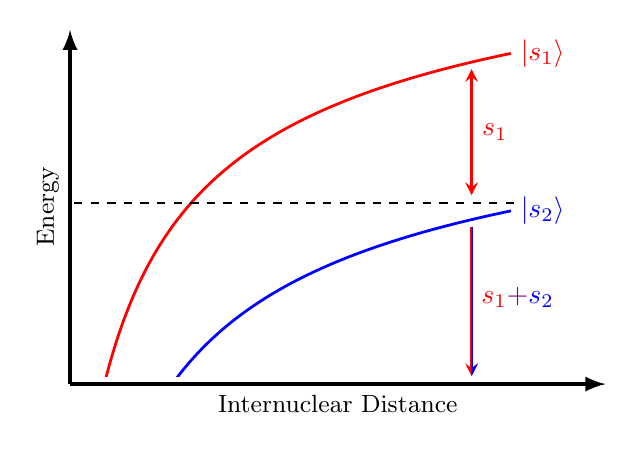
\begin{tikzpicture}
  \begin{scope}
    \clip (0.825, -2.1 - 5 / 2) rectangle (6cm, -0.5cm + 1pt);
    \draw[line width=1,blue]
    plot[domain={1}:{4},variable=\x,samples=1000] ({1.5 * \x}, {-5 / sqrt(\x)});
    \draw[line width=1,red]
    plot[domain={0.55}:{4},variable=\x,samples=1000] ({1.5 * \x}, {2 - 5 / sqrt(\x)});
  \end{scope}
  \node[red,right] at (6, -0.5) {$|s_1\rangle$};
  \node[blue,right] at (6, -2.5) {$|s_2\rangle$};
  \draw[dashed] (0.45, -2.4) -- (6.1, -2.4);
  \draw[red,<->,>=stealth,line width=1] (5.5, -0.7) -- node[right] {$s_1$} (5.5, -2.3);
  \draw[red,->,>=stealth,line width=1] (5.5, -2.7) -- (5.5, -4.6);
  \begin{scope}
    \clip (5.5, -2.5) rectangle (6, -4.8);
    \draw[blue,->,>=stealth,line width=1] (5.5, -2.7) -- (5.5, -4.6);
  \end{scope}
  \node[right] at (5.5, -3.6)
  {\textcolor{red}{$s_1$}\textcolor{red!50!blue}{$+$}\textcolor{blue}{$s_2$}};
  % Total
  \draw[line width=1.5,->] (0.4, -4.7) --  node[below] {\small Internuclear Distance} (7.2, -4.7);
  \draw[line width=1.5,->] (0.4, -4.7) --  node[above,rotate=90] {\small Energy} (0.4, -0.2);
\end{tikzpicture}
\end{document}
